% ============================================================
%  孟凡腾 — 简历（风格 C · 现代商务顶栏 / 深蓝＋琥珀）
%  数据沿用 cv_CN（不覆盖既有文件）。
%  编译：xelatex cv_CN-business.tex
% ============================================================
\documentclass[10.5pt,a4paper]{ctexart}

\usepackage[margin=1.6cm,top=0.0cm,bottom=1.5cm]{geometry}
\usepackage{xcolor}
\usepackage{graphicx}
\usepackage{array}
\usepackage{titlesec}
\usepackage{enumitem}
\usepackage[hidelinks,pdftitle={Fanteng Meng -- CV},pdfauthor={Fanteng Meng}]{hyperref}

% ---------------- 调色 ----------------
\definecolor{navy}{RGB}{15,42,88}
\definecolor{navy2}{RGB}{26,60,118}
\definecolor{amber}{RGB}{231,150,26}
\definecolor{ink}{RGB}{45,46,50}
\definecolor{graytext}{RGB}{110,115,122}
\definecolor{light}{RGB}{237,241,248}

% 章节标题：导航蓝 sans 标题 ＋ 左琥珀竖线
\titleformat{\section}
  {\large\sffamily\bfseries\color{navy}}
  {}{0.5em}
  {\colorbox{amber}{\rule[-0.25ex]{0.14em}{2.0ex}\hspace{0.55em}}\kern0.2em}
  [\vspace{-0.3em}{\color{navy!22}\rule{\textwidth}{0.8pt}}]
\titlespacing*{\section}{-2pt}{13pt}{7pt}

\newcommand{\navypill}[1]{\colorbox{navy}{\kern0.4em\strut\footnotesize\sffamily\bfseries\color{white}#1\kern0.4em}}
\newcommand{\ambpill}[1]{\colorbox{amber}{\kern0.4em\strut\footnotesize\sffamily\bfseries\color{white}#1\kern0.4em}}

% ---------------- 顶部商务横幅 ----------------
\newcommand{\makecvheader}{%
  \setlength\fboxsep{0pt}\noindent
  \colorbox{navy}{%
    \begin{minipage}{\textwidth}%
      \color{white}
      \begin{minipage}[t]{0.70\textwidth}
        \hspace{1.2em}\vspace{1.4em}
        {\fontsize{31}{34}\selectfont\sffamily\bfseries 孟凡腾}\ \ 
        {\color{white!75}\large Fanteng Meng}\par\vspace{0.6em}
        \hspace{1.5em}{\color{amber}\rule{0.5ex}{0.9ex}}\kern0.5em
        {\color{white!95}\sffamily 安全科学与工程 · 博士研究生}\par\vspace{0.7em}
        \hspace{1.5em}{\footnotesize\color{white!72}无人机智能巡检 · 机器视觉 · 深度学习 · 低空感知}\par
        \vspace{1.0em}
      \end{minipage}%
      \hfill
      \begin{minipage}[t]{0.28\textwidth}
        \raggedleft\vspace{1.2em}
        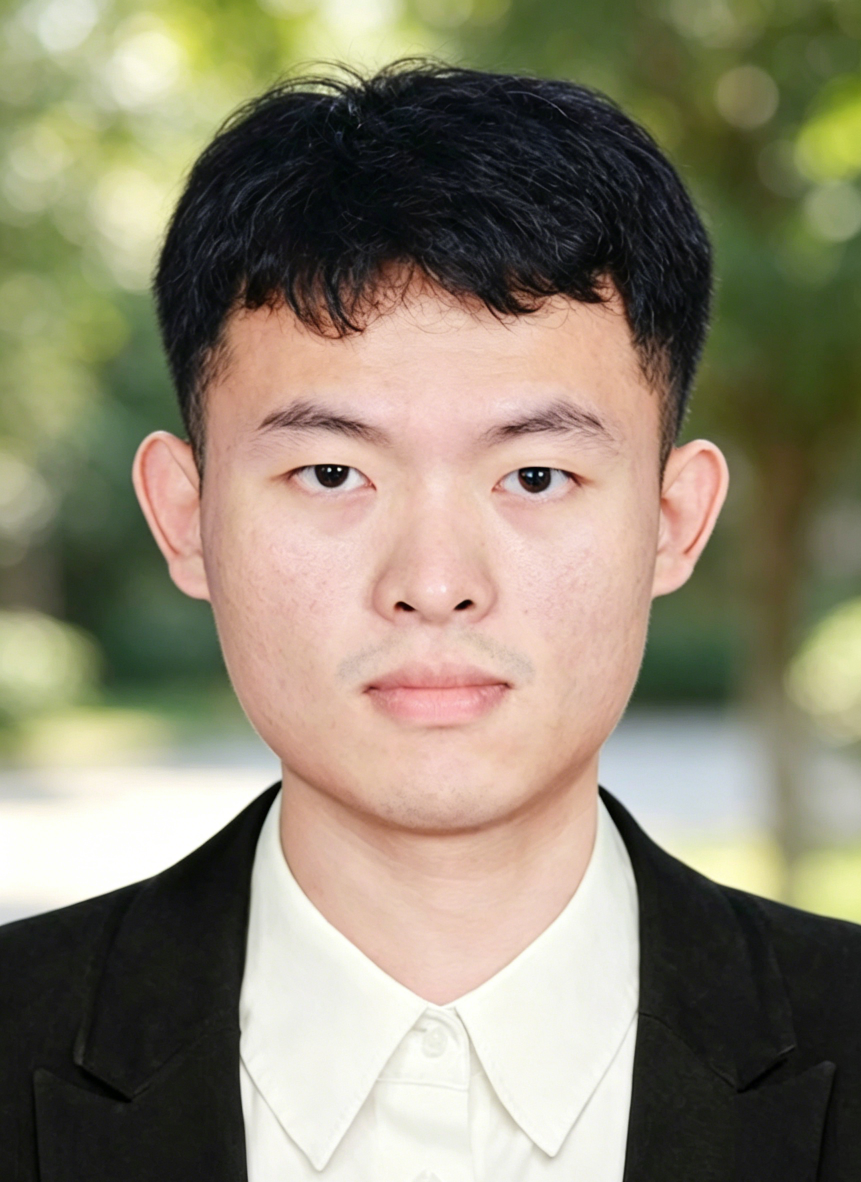
\includegraphics[width=2.65cm,height=2.65cm,keepaspectratio]{../images/photo-202601-square.png}
        \par\vspace{1.1em}
      \end{minipage}%
      \par\vspace{0.2em}
      \noindent\hspace{1.2em}\small\sffamily
      \href{mailto:ftmeng@bjtu.edu.cn}{\color{white}ftmeng@bjtu.edu.cn}
      \hspace{1.4em}$\cdot$\hspace{1.2em}
      \href{https://ft115.github.io}{\color{white}ft115.github.io}
      \hspace{1.4em}$\cdot$\hspace{1.2em}
      \href{https://scholar.google.com.hk/citations?user=Yq5wnc8AAAAJ}{\color{white}Google Scholar}
      % 单位写在第二行末
      \\[0.5ex]
      \hspace{1.2em}{\footnotesize\color{white!80}北京交通大学 · 先进轨道交通自主运行全国重点实验室 / 交通运输学院（智能系）}
      \par\vspace{1.2em}
    \end{minipage}%
  }%
  \par\vspace{1.1em}
}

\begin{document}
\makecvheader

% ============ 教育 ============
\section{教育经历}

\noindent\textbf{博士 · 安全科学与工程}\hspace{0.8em}\navypill{2023 — 至今}\par\vspace{0.3em}
\begin{itemize}[leftmargin=1.1em,label=\textcolor{amber}{$\bullet$},itemsep=1.5pt]
  \item 北京交通大学 · 先进轨道交通自主运行全国重点实验室 / 交通运输学院（智能系）
  \item 导师：秦勇 教授 · 硕博连读
\end{itemize}
\vspace{0.5em}
\noindent\textbf{硕士 · 交通运输规划与管理}\hspace{0.8em}\navypill{2022 — 2023}\par\vspace{0.2em}\noindent\small 北京交通大学
\vspace{0.5em}
\noindent\textbf{本科 · 交通运输}\hspace{1.2em}\navypill{2018 — 2022}\par\vspace{0.2em}\noindent\small 石家庄铁道大学

% ============ 方向 ============
\section{研究方向}
\noindent 无人机智能巡检　·　轨道交通机器视觉与深度学习　·　边缘计算　·　三维重建与点云分析

% ============ 论文 ============
\section{代表性论文}
{\footnotesize\sffamily\color{navy}* 通讯作者；\# 共同第一作者。}
\begin{enumerate}[label=\arabic*.,labelsep=0.5em,leftmargin=1.9em,itemsep=4pt,topsep=3pt]
  \item \textbf{Meng, F.}, Qin, Y.$^*$, Wu, Y.$^*$, et al.\ ``SRLF: Sparse Representation Learning Framework for Railroad Surrounding Potential Risk Perception Using UAV Imagery.'' \textit{IEEE Trans.\ Intell.\ Transp.\ Syst.}, 2025.\\
  {\footnotesize\color{graytext}IEEE T-ITS · 中科院 1 区 TOP · 5 年 IF 10.403}
  \item \textbf{Meng, F.}, Qin, Y.$^*$, Wu, Y.$^*$, Shao, C., Yang, H., Jia, L.\ ``Automatic Risk Level Evaluation System for Potential Environmental Hazards along High-speed Railroad Using UAV Aerial Photograph.'' \textit{Expert Syst.\ Appl.}, 2025.\\
  {\footnotesize\color{graytext}Expert Systems with Applications · 中科院 1 区 TOP · 5 年 IF 8.995}
  \item \textbf{Meng, F.}, Qin, Y.$^*$, Wu, Y.$^*$, Shao, C., Jia, L.\ ``A Subtle Defect Recognition Method for Catenary Fastener in High-speed Railroad Using Destruction and Reconstruction Learning.'' \textit{Adv.\ Eng.\ Inform.}, 2024.\\
  {\footnotesize\color{graytext}Advanced Engineering Informatics · 中科院 1 区 TOP · 5 年 IF 11.204}
  \item Wu, Y.$^\#$, \textbf{Meng, F.}$^\#$, Qin, Y.$^*$, Qian, Y.$^*$, Xu, F., Jia, L.\ ``UAV Imagery Based Potential Safety Hazard Evaluation for High-speed Railroad Using Real-time Instance Segmentation.'' \textit{Adv.\ Eng.\ Inform.}, 2023.\\
  {\footnotesize\color{graytext}Advanced Engineering Informatics · 中科院 1 区 TOP · 5 年 IF 11.204}
  \item Wu, Y.$^\#$, \textbf{Meng, F.}$^\#$, Qin, Y.$^*$, Qian, Y.$^*$, Liu, Z., Zhao, W.\ ``Automated Anomaly Detection of Catenary Split Pins Using Unsupervised Learning.'' \textit{Autom.\ Constr.}, 2024.\\
  {\footnotesize\color{graytext}Automation in Construction · 中科院 1 区 TOP · 5 年 IF 13.598}
  \item \textbf{孟凡腾}，秦勇$^{*}$，崔京，等.\ ``铁路外部环境无人机图像未知风险检测方法.'' \textit{航空学报（Acta Aeronautica et Astronautica Sinica）}, 2025.\\
  {\footnotesize\color{graytext}《航空学报》· 中文权威期刊 · 卓越行动计划 T1 · EI}
  \item 秦勇$^{*}$，\textbf{孟凡腾}$^{\#}$，张紫城，等.\ ``轨道交通基础设施自主无人机智能巡检体系框架及其技术发展综述.'' \textit{北京交通大学学报}, 2025.\\
  {\footnotesize\color{graytext}《北京交通大学学报》· 北大核心 · CSCD}
\end{enumerate}

% ============ 工程 ============
\section{代表性工程实践}
\noindent\textbf{高速铁路全自动无人机智能巡检系统}\hspace{0.6em}\ambpill{首套}\par\vspace{0.2em}
\begin{itemize}[leftmargin=1.1em,label=\textcolor{amber}{$\bullet$},itemsep=1.5pt]
  \item 国内外首套高速铁路无人机自主智能巡检系统，规模应用近百公里。
  \item 国家重点研发计划核心研究人员；设计 3 项原创视觉算法（召回率 >96%）。
  \item 部署 6 架巡检无人机 + 4 套自动化机巢；较人工巡检效率提升 10 倍以上。
\end{itemize}
\vspace{0.5em}
\noindent\textbf{青藏铁路桥梁与落石灾害无人机智能巡检}\par\vspace{0.2em}
\begin{itemize}[leftmargin=1.1em,label=\textcolor{amber}{$\bullet$},itemsep=1.5pt]
  \item 平均海拔 3000+ 米自主飞行巡检。
  \item 全栈技术研发：自主飞行控制、摄影测量三维重建、点云分割。
  \item 多期点云配准与落石形变检测，服务高原铁路运营安全。
\end{itemize}
\vspace{0.5em}
\noindent\textbf{铁路钢桁梁桥无人机全覆盖巡检与涂层缺陷评估}\par\vspace{0.2em}
\begin{itemize}[leftmargin=1.1em,label=\textcolor{amber}{$\bullet$},itemsep=1.5pt]
  \item GNSS 拒止下大跨度铁路钢桥飞行巡检。
  \item 设计覆盖桥顶、桥侧及复杂桥底区域的避障巡检航线。
  \item 端到端流程：涂层缺陷识别 → 量化分级 → 缺陷空间溯源。
\end{itemize}

% ============ 专利 ============
\section{专利}
\noindent\textbf{已授权专利}
\begin{enumerate}[label=\arabic*.,labelsep=0.5em,leftmargin=1.9em,itemsep=2pt,topsep=2pt]
  \item Autonomous UAV Based Intelligent Inspection System for Equipment, Facilities, and the Environment along Railway Lines and Method Thereof.{\ \footnotesize\sffamily\color{amber}（美国发明专利）}
  \item 基于无人机图像的铁路环境隐患识别与风险等级评估方法
  \item 用于卫星拒止下交通设施巡检的无人机航线生成方法
  \item 跨模态自适应匹配的激光雷达与相机的在线外参标定方法及系统
\end{enumerate}
\vspace{0.3em}\noindent\textbf{已公开专利申请}
\begin{enumerate}[label=\arabic*.,labelsep=0.5em,leftmargin=1.9em,itemsep=2pt,topsep=2pt]
  \item 用于无人机遥感图像的铁路沿线环境未知风险识别方法
  \item 一种用于铁路接触网的开口销缺陷精细化识别方法
  \item 铁路钢桁架桥涂层锈蚀检测评估方法及系统
\end{enumerate}

% ============ 荣誉 ============
\section{荣誉与获奖}
\begin{flushleft}
\begin{tabular}{@{}l@{\hspace{1.1em}}l@{}}
\navypill{2024} & 第十四届“挑战杯”中国大学生创业计划竞赛“一带一路”国际邀请赛 · 银奖\\[0.6ex]
\navypill{2024} & “青创北京”首都大学生挑战杯创业计划竞赛 · 银奖\\[0.6ex]
\navypill{2022} & 北京交通大学暑期深度学习训练营 · 二等奖\\[0.6ex]
\navypill{2021} & 中国交通优秀学子 · 一等奖\\[0.6ex]
\navypill{2021} & 第七届全国大学生工程训练综合能力竞赛 · 省级一等奖\\[0.6ex]
\navypill{2021} & 省级三好学生\\[0.6ex]
\navypill{2020} & 第十二届全国大学生数学竞赛 · 省级一等奖\\[0.6ex]
\navypill{2020} & 第七届全国大学生物理竞赛 · 省级一等奖\\
\end{tabular}
\end{flushleft}

% ============ 服务 & 技能 ============
\section{学术服务}
\noindent\textbf{期刊审稿人}\quad \textit{IEEE Trans.\ Intell.\ Transp.\ Syst.}(T-ITS)、\textit{Adv.\ Eng.\ Inform.}(AEI)、\textit{Expert Syst.\ Appl.}(ESWA)

\section{专业技能}
\noindent 编程语言与框架：Python · C++ · Matlab · PyTorch \quad$|$\quad 系统：Linux、ROS     \quad$|$\quad 视觉：OpenCV \quad$|$\quad 机载：DJI-PSDK

\end{document}
